
\textit{In this chapter, we will talk about what is Monte Carlo tree search is and how it applied to the game of Go.}
\\

\textit{First we will talk about the Monte Carlo part and the tree search part separately, then explain how the fusion work.}
\\

\textit{The second section is about the benefits and drawbacks of MCTS}
\\

\textit{Thirdly, we will see the big dilemma of MCTS : Exploitation versus Exploration}
\\

\textit{And last but not least, there is a part where we see the application of MCTS to the game of go and what are the actual heuristics used today. }

\section{Monte Carlo tree search}

\subsection{Monte Carlo}

Monte Carlo methods are a big set of algorithms that works by using a repeated random sample to estimate a solution. They are widely used in a lot of domains like Physics, computational biology, computer graphics or science, Artificial intelligence, even economics. 
\\

There is four steps to a Monte Carlo algorithm : 

\begin{itemize}
\item Define a domain of inputs
\item Generate random value over the domain following a probability distribution
\item Compute the result
\item Use the result to get what you wanted
\end{itemize} 

We'll show this four steps through an example : the computation of $\pi$. How to estimate $\pi$ with a random generation. 

\begin{itemize}
\item Define a domain of inputs : the square of coordinates (0,0),(1,0),(0,1) and (1,1).
\item Generate random value over the domain following a probability distribution : Generate points randomly into this square. 
\item Compute the result : compute $x$ where $x = \frac{In}{Total}$ and where $Total$ is the number of points generated and $In$ is the number of points inside the circle of radius 1. 
\item Use the result to get what you wanted : With a sufficient high number of $Total$ we can approximate thanks to the law of big numbers and assume


$$\frac{In}{Total}= \frac{\textrm{area of the quarter of the circle}}{\textrm{area of the square}}$$

 As the area of the circle is $ \pi*1^2$ , the quarter is $\frac{\pi}{4}$. And so we got our final equation : 

$$
\frac{In}{Total}=\frac{\pi}{4}
$$
\end{itemize} 

Results have show that with enough tries, we can get really close to the real value of $\pi$. 

\subsection{Tree search}
In this section we will explain the basics of tree search in artificial intelligence, some techniques already used and how they differ of MCTS. 
\\

A tree is an abstract representation of a game. Each node represents a state of the game. The root is the initial state. Then there is one children for each move possible since that state. 
\\

Some assumptions need to be made : 
\begin{itemize}
\item The game is turn by turn, not in real time. 
\item Two players.
\item Fully observable

\end{itemize}

Here's an example of a tree for a game where two players flip a coins and try to maximize the number of heads. The game begin with 0 heads for each player and the first to play is the blue player. Either the coin is head then the game move to the node with 1 head either it's tail then the state is the 0 blue node. Then the red player plays and so on. 
\begin{center}
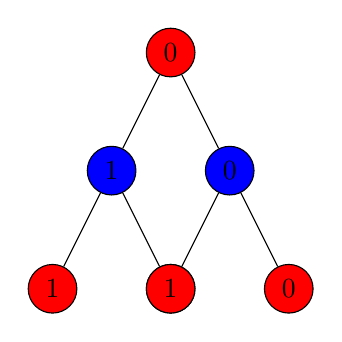
\begin{tikzpicture}
\node[circle,draw,fill=red](z){$0$}
  child{ node[circle,draw,fill=blue]{1} child{node[circle,draw,fill=red] {1}} child{node[circle,draw,fill=red] {0}} }
  child{
    node[circle,draw,fill=blue]{0} child{node[circle,draw,fill=red] {1}} child{node[circle,draw,fill=red] {0}} };
\end{tikzpicture}
\end{center}
\subsubsection{Mini-max}

The minimax algorithm is an algorithm in artificial intelligence games. It will try to win by giving to each state of the game a score. Following the name of the algorithm player one
 will try to maximize the score, while the other will try to minimize it. So a bigger score is a better situation for player one. Each action or move will impact the score. Thus, the algorithm will choose the action that eventually bring him into the best state for him, assuming the other player plays the best moves he can. In the best cases, the algorithm continue to search the tree until he finds a finished won situation but as it's not always possible to compute such depth, he limits himself to the best score. 
\\

 \begin{verbatim}
 function minimax(node, depth, maximizingPlayer)
    if depth = 0 or node is a terminal node
        return the heuristic value of node
    
    if maximizingPlayer
       bestValue := -minus infinity
    else
       bestValue := infinity
    
    for each child of node
        val := minimax(child, depth - 1, !maximizingPlayer)
        if maximizingPlayer
            bestValue := max(bestValue, val)
        else
            bestValue := min(bestValue, val)
    return bestValue
 \end{verbatim}
 
 This is the basis principle of a minimax search. There are several benefits to this technique but it suffers some major drawbacks. 
 
 \begin{itemize}
 \item It needs to explore in breadth first search, meaning all nodes from the top, depth after depth. In some case it's just impossible. The complexity of the minimax is $(b^d)*e$ where b is the branching factor(number of possible moves), d is the depth wished, and e is the complexity of the evaluate function. In the case of Go by example, the initial branching factor is 361. We easily understand that such a complexity wouldn't be applicable.
 \item The algorithm needs an evaluate function which will return a value, a score for a node. It needs a deep knowledge of the game to produce a correct and precise heuristic when it's possible which is not always the case. In the case of Go, it's practically impossible to always being able give a value to a board, or even to say which player is at an advantage. The game can change on a single move. 
 \end{itemize}

\subsection{Monte Carlo and Tree search combined}

We will now see how to combine these two principle to form the Monte Carlo tree search. The idea is relatively simple. As the total tree of the game is far to big to be computed, it will only compute the necessary tree. Which means computing the tree node by node, with information on what node build next. And in the end, there will be a far smaller tree indicating the best moves. In the following sections, the process of building the tree will be detailed. 

\subsubsection{Four Steps}
This section will present with the help of figure how one execution of the Monte Carlo tree search occur, through the four steps. Two names are given each time for the steps, it doesn't mean something different. It's just that theses steps are not called the same everywhere. The two names found were put to help a reader. We present an initial tree that already was partially built. There's two colors, one for each player. The first number in the nodes is the number of times the owner of the root node won passing by that state. The second is the number of times the algorithm passed by that state. By example if you take right leaf node, we can see the red players won 0 times on 4 passages. 
\begin{center}
\begin{tikzpicture}[->,>=stealth',level/.style={sibling distance = 5cm/#1,
  level distance = 1.5cm}] 
\node [arn_n] {5/10}
    child{ node [arn_r] {4/6} 
            child{ node [arn_n] {0/2}}
            child{ node [arn_n] {4/4}
							child{ node [arn_r] {1/1}}
							child{ node [arn_r] {3/3}}
            }                            
    }
    child{ node [arn_r] {1/4}}
; 
\end{tikzpicture}
\end{center}

\subsubsection{Selection or descent}
The first step is the selection, the algorithm will select node after node the best moves for him. The criteria of best moves can vary, and the different strategies will be explain further. For the moment, it simply selects the one with the best ratio won/played. The moves chosen are highlighted by being in diamond shape. 

\begin{center}
\begin{tikzpicture}[->,>=stealth',level/.style={sibling distance = 5cm/#1,
  level distance = 1.5cm}] 
\node [arn_nc] {5/10}
    child{ node [arn_rc] {4/6} 
            child{ node [arn_n] {0/2}}
            child{ node [arn_nc] {4/4}
							child{ node [arn_r] {1/1}}
							child{ node [arn_rc] {3/3}}
            }                            
    }
    child{ node [arn_r] {1/4}}
; 
\end{tikzpicture}
\end{center}
\subsubsection{Expansion or growth}
Once the selection phase reach either a terminal state of the game or a leaf node of the tree built, we arrive at the expansion phase.If this is not a terminal state, the basic strategy from this point is to select a random move and add it to the tree with a 0/0 statistics. 

\begin{center}
\begin{tikzpicture}[->,>=stealth',level/.style={sibling distance = 5cm/#1,
  level distance = 1.5cm}] 
\node [arn_nc] {5/10}
    child{ node [arn_rc] {4/6} 
            child{ node [arn_n] {0/2}}
            child{ node [arn_nc] {4/4}
							child{ node [arn_r] {1/1}}
							child{ node [arn_rc] {3/3}
								   child{ node [arn_nc] {0/0}}							
							}
            }                            
    }
    child{ node [arn_r] {1/4}}
; 
\end{tikzpicture}
\end{center}

\subsubsection{Simulation or roll-out}

From this state of the game the simulation step plays random move one after another for each player until reaching a final state. 

\subsubsection{Backpropagation or update}
Once a final state is reached, it computes who's the winner and then, node by node, update the value of the tree. In the example, the black player will win. It will then update all the nodes on the path from the leaf node to the root. 

\begin{center}
\begin{tikzpicture}[->,>=stealth',level/.style={sibling distance = 5cm/#1,
  level distance = 1.5cm}] 
\node [arn_nc] {6/11}
    child{ node [arn_rc] {5/7} 
            child{ node [arn_n] {0/2}}
            child{ node [arn_nc] {5/5}
							child{ node [arn_r] {1/1}}
							child{ node [arn_rc] {4/4}
								   child{ node [arn_nc] {1/1}}							
							}
            }                            
    }
    child{ node [arn_r] {1/4}}
; 
\end{tikzpicture}
\end{center}

The execution is now finished. There is two possibilities, either there's still time, and the algorithm can process one more, or the algorithm must choose a move and will select by example the one with the best ratio, here the move on the left, 5/7. Indeed, by choosing that, he got 5 out of 7 chance to win, where in the other case, he would have loose for sure. 
\\

Thus, it's the principle of the Monte Carlo tree search. Only searching where it's interesting. By doing enough iterations, like with the computation of $\pi$, we can compute a tree that will be big enough to be statistically representative. 
\\

Now we will explore the different strategies possible for each steps. 

\subsection{Basic Strategies for each step}

There are several strategies for each step. To understand well notably the strategies for the selection step, it must be clear that there's a big dilemma in the application of Monte Carlo tree search. The problem is between two elements : Exploitation, which means taking profits of what you already know, and Exploration, which means go see elsewhere if there's not something better. When you exploit, you can't explore and the inverse is also true. So there's always that question : "Am I on the right path ? Should I go further on it, or should I try something else". 
The following section, with the strategies for the selection step will enlighten some answer. 

\subsubsection{Selection - Objective Monte Carlo}

The goal of this technique is to compute a fairness function for each move. It will attribute a probability to each possible move and will then select randomly one in the possible, following the probabilities found. The fairness function reflect the balance between the exploitation and exploration. It will be shown here. 
\\

First the fairness function for each move m is the following, where $n_p, n_m$ is the count of visit for the parent of m, for m respectively, PM is the ensemble of possible moves and U(x) is the urgency function of x. 
$$
f_m = \frac{n_p U(m)}{n_m \sum\nolimits_{j \in PM} U(j)}
$$

U(x) is a function that allows estimating if a move must be played. To be exact, it's : 
$$
U(m) = erfc(\frac{v_0 -v_m}{\sqrt{2}\sigma_m}
$$
$v_x$ is the value of the node x

0 is the best move. 

$\sigma_x$ is the standard deviation of x. The standard deviation for a discrete variable with the same chance for each value is : 

$$ 
\sigma_x 	= \sqrt{\frac{1}{N} \sum\limits_{i=1}^{N} (x_i-\mu_i)^2}
$$

TODO

\subsubsection{Expansion}
TODO
\subsubsection{Simulation}
TODO
\subsubsection{Backpropagation}
TODO

\subsubsection{Selection of the final move}
Todo

\subsection{Benefits and Drawbacks}

\subsubsection{Benefits}

Monte Carlo tree search draw a lot of advantages from his special technique of using tree search and random simulations. 
\begin{itemize}
\item Aheuristic : There's absolutely no need for heuristic in the refined version of Monte Carlo tree search. All you need to know about the game is the possible moves from a state, and the winning situations for a player. Except that, which are the basic rules, you don't need to know how to play, to be a professional or having a really good vision of how to play the game to implement an artificial intelligence player.
\item Asymmetric : In place of having a gigantic tree, taking an incredible amount of space, there's only the needed tree, much much smaller than the complete one. As it's build only depending of the needs, it can be completely asymmetric. 
\item Non time limited. One of the beautiful part of the Monte Carlo tree search is that you don't need a specific amount of time. The output of the program is not binary depending of the time. Some algorithm will take a certain amount of seconds or minutes, then deliver an answer. Here, the algorithm can always, at any time deliver an answer. Of course, the more time is given, the better the answer. But it allows stopping the search, either after a certain time or a number of iterations trough the four steps. 
\item The basic version of Monte Carlo tree search can be implemented really simply. It's his efficient adaptation to complex games that makes it difficult. 
\end{itemize}

\subsubsection{Drawbacks}

Here's come the second part about the big dilemma talked sooner.  There are several moments, as seen in the strategies, that give difficult choices. By example, in the simulation step, if it's too complicated, it will take too much time, leading to fewer iterations and so to not statistically representative results. On the other hand, if it's too simple, it won't reflect real plays, and moreover, it can create the same problem than a complicated heuristic, as it do a lot of random bad plays, it won't represent a good player, even with a high number of play. 

There are some heuristics that were thought for this, one of them, the MC-RAVE will be explained later for the Go. 


\section{Monte Carlo tree search applied to Go}

Before the introduction of Monte Carlo, the field of artificial intelligence in go was kinda stuck. The programmers couldn't make a bot player better than an average good human player. Then, with Monte Carlo, the level of all bot jump trough the sky as we can see on the representative figure
\begin{center}
\includegraphics[scale=0.5]{perf.jpg}
\end{center}
\subsection{Improvement}
Here we will present some heuristic specifically applied to the case of the Monte Carlo tree search on the game of go. 
The first one is general and the second one is for the expansion step. 

\subsubsection{MC-RAVE}

The idea behind the MC-Rave is rather simple. The basic Monte Carlo tree search algorithm always consider a move dependently from a state. But in Go, they are a lot of situations where a part of the state won't influence the quality of a move. By example there's really little chance that the stones put in a corner of the board will affect the stones in the other corner. That's where come from the idea of AMAF, or all moves as first. Thus, each move will have a rating consisting of $ \frac{\tilde{W}(a)}{\tilde{N}(a)} $ where $N(a)$ is a number of simulation where the move $a$ was played at any time, and $W(a)$ is the number of times the black player won. 
\\

Once we got Amaf value for each move, we could make it play with that for all game, but as the games progress, there's more and more influence from the state of the board. Thus, the MC-Rave heuristic corrects that by giving less weight to the AMAF value as the number of plays increase. Here's the equation for the Value of a move "a" from a state s. 

$$
 \tilde{V}(s,a) = (1-\beta (s,a)) \frac{W(s,a)}{N(s,a)}+ \beta (s,a) \frac{\tilde{W}(a)}{\tilde{N}(a)}
$$

Where $\beta$ is a parameter decreasing from 1 to 0 as the game progress, and so the visit count $N(a)$ increases. 

\subsubsection{Bradley and Terry model}

Suppose some people in a competition. This model assign to each player a strength $\alpha$ then it predicts the chance to win of the player i against the player j to :
$$
P(i vs j) = \frac{\alpha_i}{\alpha_i+\alpha_j}
$$
There's also possibility to play in team : 

$$
P(1+2 vs 3+4) = \frac{\alpha_1*\alpha_2}{\alpha_1*\alpha_2+\alpha_3*\alpha_4}
$$

As in go there are several types of moves, each move has different feature. Here's a possible list :

\begin{itemize}
\item Atari
\item Distance of x of previous move
\item Secure group
\item Next to group/alone
\end{itemize}

The idea is to give to each of theses features a strength $\alpha$ so the probability of a move a from state s :

$$
P(s_a)= \frac{\prod\limits_{features\; i\; in\; s_a}\alpha_i}{\sum\limits_{legal\; moves\; from\; s}(\prod\limits_{feature\; i\; in\; s_j}\alpha_i)}
$$

Then we can compute this probability for all legal moves. To limit the search, progressive widening is used. In a lot of case in A.I, the algorithm pruned the search space, here's it's the opposite. The goal is to un-pruned as plays increase. The algorithm will look into the T best moves following the Bradley and Terry model The following formula is used by the developer of AYA, a big and well known go program, where's n is the number of plays, and $\mu$ a parameter : 

$$
T = 1+ \frac{\log n}{\log \mu}
$$